\begin{remark}
    Section made from lectures done by Dr.\ Emma Bland. Other sources are \citet{BrekkeAsgeir2013Potu} --- chapter 3 part 1 to 7, chapter 6.5 and chapter 7.1 --- and \citet{TwymanR.M.GEAS}.
\end{remark}

\section{Sources to the Earth's magnetic field}
Sources to the magnetic field of the Earth are (1) the core/main field (\cref{fig:L3_contributor1,fig:L3_contributor2}). This come from a self-sustaining dynamo action in the Earth's outer liquid core and contributes to more than 95\% of total field strength. The field strength is \(\approx\SI{25}{\micro\tesla}\) at equator and \(\approx\SI{65}{\micro\tesla}\) at the poles and the field can be described by a simple dipole model, with axis tilted \(\sim\SI{11}{\degree}\) from Earth’s rotation axis. This model have an error of \(\sim 30\% \) for \(R<4R_E\), while closer to the Earth the error is within \(10\% \). Another source is the (2) crustal field (\cref{fig:L3_contributor3}). This come from ferromagnetic minerals in the Earth’s crust and the contribution is typically a few hundred \si{\nano\tesla}, but up to thousands of \si{\nano\tesla} at some locations (can affect compasses). The (3) external field (\cref{fig:L3_contributor3}) is a third contribution. This arises from electric currents flowing in ionosphere and magnetosphere. Under quiet conditions it gives only fractions of \si{\nano\tesla} while a large geomagnetic storm can give thousands of \si{\nano\tesla}. Finally a fourth source is (4) electromagnetically induced fields (\cref{fig:L3_contributor3}). This is generated by currents induced in the crust and upper mantle by temporal fluctuations in the external field and gives up to tens of \si{\nano\tesla}.
\begin{figure}[ht]
	\centering

    \begin{subfigure}[t]{0.3\textwidth}
        \centering
        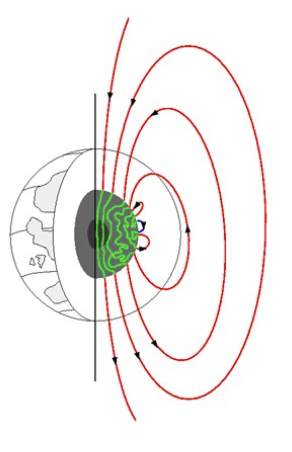
\includegraphics[width=.9\linewidth]{bilder/L3_earth_four_1.png}
        \caption{}\label{fig:L3_contributor1}
    \end{subfigure}
	\begin{subfigure}[t]{0.3\textwidth}
		\centering
		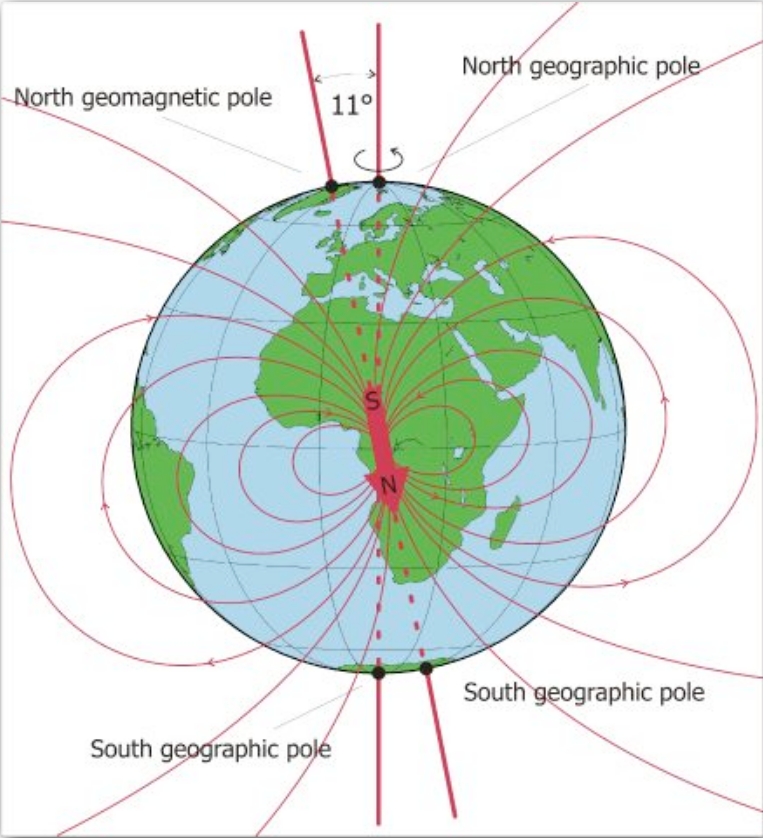
\includegraphics[width=.9\linewidth]{bilder/L3_earth_four_2.png}
		\caption{}\label{fig:L3_contributor2}
    \end{subfigure}
    \begin{subfigure}[t]{0.3\textwidth}
		\centering
		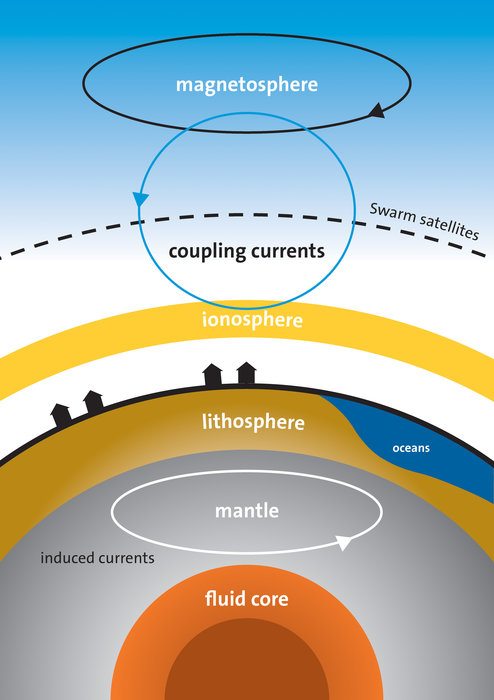
\includegraphics[width=.9\linewidth]{bilder/L3_earth_four_3.jpg}
		\caption{}\label{fig:L3_contributor3}
	\end{subfigure}

	\caption{The different contributors to the magnetic field.}\label{fig:L3_earth_magnetic_four_contributors}
\end{figure}
\begin{figure}[ht]
    \centering
    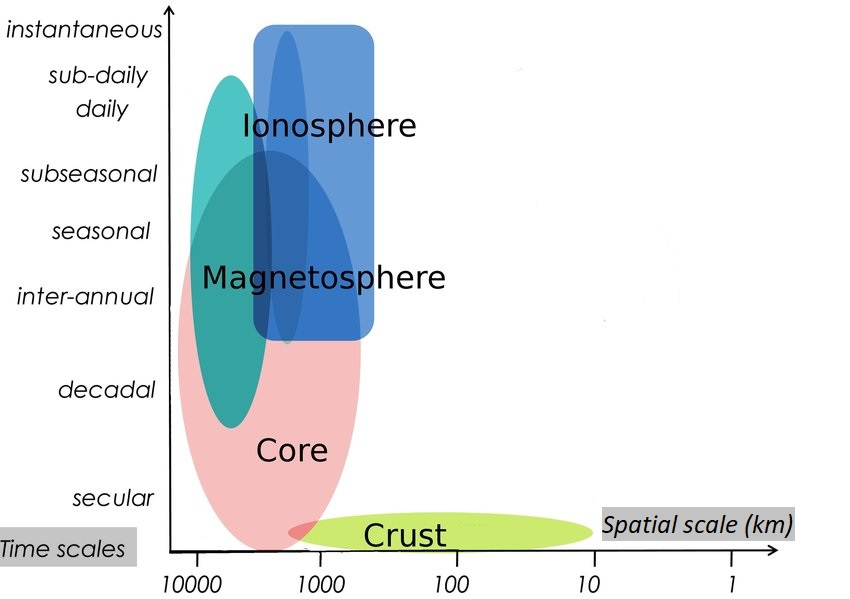
\includegraphics[width=.6\linewidth]{bilder/L3_earth_magnetic_contributors.jpg}\label{fig:L3_earth_magnetic_contributors}
    \caption{Spatial and temporal variations in the Earth's magnetic field. Source: }
\end{figure}

\section{Magnetic field in equation form}
We neglect currents flowing between Earth's surface and space. Outside the Earth:
\begin{equation*}
    \gf{j}=0\quad\Rightarrow\quad\nabla\times\gf{B}=0
\end{equation*}
where we have used \cref{eq:MHD_5}. We must then have a magnetic potential \(\Phi_m\) such that \(\gf{B}=-\nabla\Phi_m\). Also \(\nabla\cdot\gf{B}=0~~\therefore \nabla^2\Phi_m=0\).

We will now write the components of \(\gf{B}\) in spherical coordinates, as
\begin{equation}
    \nabla\Phi_m=\p{r}{\Phi_m}\widehat{\f{r}}+\frac{1}{r}\p{\theta}{\Phi_m}\widehat{\f{\theta}}+\frac{1}{r\sin\theta}\p{\phi}{\Phi_m}\widehat{\f{\phi}}
\end{equation}
where \(\gf{B}_r=-\p{r}{\Phi_m}\), \(\gf{B}_\theta=-1/r\p{\theta}{\phi}\) and \(\gf{B}_\phi=-1/r\sin\theta\p{\phi}{\phi}\). However, we can't describe the geomagnetic field as a simple analytical function. We usually find the magnetic potential \(\Phi_m\) from a set of observations of \(\gf{B}\). To achieve this, we can expand \(\Phi_m\) into a series of spherical harmonics in polar coordinates as
\coloredeq{eq:most_important_one}{\Phi_m\left(r,\theta,\phi,t\right)=R_E\sum_{n=0}^\infty\left(\frac{R_E}{r}\right)^{n+1}\sum_{m=0}^nP_n^m (\cos\theta)\left[g_n^m\cos(m\phi)+h_n^m\sin(m\phi)\right]}
where \(R_E\) is the Earth radius, \(P_n^m(\cos\theta)\) are the normalized Legendre functions and \(g_n^m\) and \(h_n^m\) are Gaussian functions. We have used \((\theta,\phi)\) as the geographic coordinates, where \(\theta\sim \) co-latitude \(=90\degree-\)latitude.

We look at the first few coefficients:
\begin{align*}
    \left.\begin{aligned}
        n=0\\m=0
    \end{aligned}\right \}&\qquad g_0^0=0~\tn{we want no magnetic monopoles}\\
    \left.\begin{aligned}
        n=1\\m=0
    \end{aligned}\right \}&\qquad
    \left \{\begin{aligned}
        g_1^0&~\tn{main dipole term}\\
        \Phi_m&=g_1^0\cos\theta{\left(\frac{R_E}{r}\right)}^2R_E\\
        M_1&=g_1^0\frac{4\pi}{\mu_0}R_E^3
    \end{aligned}\right.\\
    \left.\begin{aligned}
        n=1\\m=1
    \end{aligned}\right \}&\qquad
    \left \{\begin{aligned}
        &g_1^1\tn{ and }h_1^1~\tn{we get an equivalent expressiona as for }g_1^0\\
        &g_1^1: M_2=\frac{4\pi}{\mu_0}g_1^1R_E^3\\
        &h_1^1: M_3=\frac{4\pi}{\mu_0}h_1^1R_E^3
    \end{aligned}\right.
\end{align*}
The result of these magnetic moments is
\coloredeq{eq:magnetic_moment}{M_0=\frac{4\pi}{\mu_0}R_E^3\underbrace{\sqrt{\left(g_1^0\right)^2+\left(g_1^1\right)^2+\left(h_1^1\right)^2}}_{H_0}}
\begin{txboxed}\emph{International Geomagnetic Reference Field (IGRF).} Coefficients updated every 5 years. Takes into considerations the effects from the inner and outer core, but not what happens in e.g.\ the ionosphere.
\end{txboxed}
\(M_0\) makes an angle with the Earth's rotation axis
\begin{equation*}
    \tan\delta=\left(\frac{\sqrt{{\left(g_1^1\right)}^2+{\left(h_1^1\right)}^2}}{g_1^0}\right)=0.17
\end{equation*}
\begin{equation*}
    \Rightarrow \delta=9.7\degree
\end{equation*}
We will now look at the magnetic field at the equator and the poles. Since \(\delta \) is small, we will assume \(M_0\) is parallel to te rotation axis
\begin{equation*}
    \Rightarrow \gf{M}_0=-M_0\f{z}
\end{equation*}
The dipole potential is then
\begin{equation*}
    \begin{aligned}
        \Phi_m&=-\frac{\mu_0}{4\pi}\gf{M}_0\cdot\nabla\frac{1}{r}\\
        &=-\frac{\mu_0}{4\pi}\frac{\gf{M}_0\cdot\gf{r}}{r^3}\\
        &=-\frac{\mu_0}{4\pi}\frac{M_0\cos\theta}{r^2}
    \end{aligned}
\end{equation*}
The components of \(\gf{B}\) can be derived from \(\Phi_m\)
\begin{align*}
    B_r&=-\p{r}{\Phi_m}=-\frac{\mu_0}{2\pi}\frac{M_0\cos\theta}{r^2}=-\frac{\mu_0M_0}{2\pi}\frac{\sin\lambda_m}{r^3}\\
    B_\theta&=-\frac{1}{r}\p{\theta}{\Phi_m}=-\frac{\mu_0}{4\pi}\frac{M_0\sin\theta}{r^3}=-\frac{\mu_0}{4\pi}\frac{M_0\cos\lambda_m}{r^3}\\
    B_\phi&=0
\end{align*}
where \(\lambda_m\) is the magnetic latitude. We find the magnitude of \(B\) to be
\coloredeq{eq:magnitude_magnetic_field}{B (r,\lambda_m)=\sqrt{B_r^2+B_\theta^2+B_\phi^2}=\frac{\mu_0}{4\pi}\frac{M_0}{r^3}\sqrt{1+3\sin^2\lambda_m}}
From earlier we had an expression for the magnetic moment in \cref{eq:magnetic_moment} which then imply
\begin{equation*}
    B(r,\lambda_m)=H_0{\left(\frac{R_E}{r}\right)}^3\sqrt{1+3\sin^2\lambda_m}
\end{equation*}
At the Earth's surface \(r=R_E\), so
\begin{align*}
    B_{\tn{pole}}&=2H_0,\quad\lambda_m=90\degree \\
    B_{\tn{equator}}&=H_0,\quad\lambda_m=0\degree
\end{align*}

\section{Magnetometers --- measuring the \(\gf{B}\)-field}
The measured components of \(\gf{B}\) are usually given in \(\gf{B}(X,Y,Z), \gf{B}(H,D,Z), \gf{B}(H,D,I)\), where \(H=\sqrt{X^2+Y^2}\) is the horizontal component, \(D=\arctan(X/Y)\) is the declination and \(I=\arctan(Z/H)\) is the inclination.
\begin{figure}[ht]
    \centering
    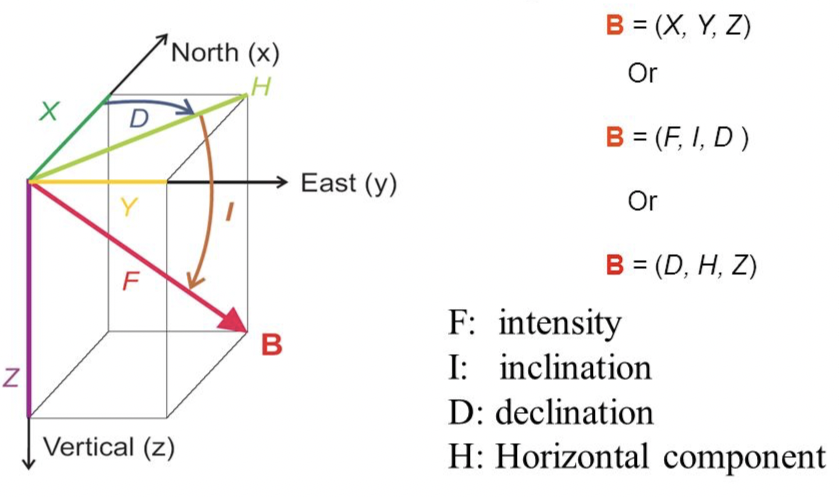
\includegraphics[width=.45\linewidth]{bilder/magnetometer_coor.png}
    \caption{Coordinate system used when measuring the geomagnetic field.}\label{fig:magnetometer_coor}
\end{figure}

\subsection{Slow variations}
The magnetic field we measure with the magnetometers can be split up into different contributors. Among the slow variations in the magnetic field we have (1) secular variations which are continuous drift in the intensity and direction of the field and the changes are noticeable over relatively short timescales (tens of years). It can be seen as a gradual monotonic decline in field intensity, about \(20\% \) over the last \(500\) years. We have also got (2) geomagnetic excursions. This is radical swings in field direction accompanied by a decrease in field strength, with a timescale of tens to thousands of years. The magnetic pole position changes by up to \SI{45}{\degree} but it is not usually recorded around the entire world. In most cases, the field regenerates with the original polarity. A (3) geomagnetic reversal is when the magnetic north and south poles are interchanged. We have had \(183\) reversals over the last \(83\) million years, with the most recent one occurring \(\num{780000}\) years ago. The occurrence is statistically random.

\subsection{Fast variations}
Fast variations are often more interesting when looking at magnetometer data. They happen on the time scales of a few minutes to several days and originate externally, e.g.\ due to currents in the ionosphere and magnetosphere. Fast variations may be a solar storms or substorms, geomagnetic pulsations or it may be solar quiet (\(S_q\)) variations. These are neutral winds that exist in the ionosphere (driven by solar heating, lunar \& solar tides). The winds will then create movement in electric charges in the E-region ionosphere, thus making current systems, and the magnetometer stations around the world can be used to track these currents. The \(X\)-component points to geographic north and at low latitudes this component have a single maximum near midday, being almost constant at night. In mid-latitude we see a decrease in the midday maximum, and at \(\sim\SI{35}{\degree}\) we see a double wave. The higher latitude have a single minimum around noon. The \(Y\)-component pointing to the east have, in the northern hemisphere, a morning maximum and afternoon minimum, with the opposite being the case for the southern hemisphere. The \(Z\)-component, which points down, have at noon a minimum in the northern hemisphere and a maximum in the southern hemisphere, with the greatest amplitudes in the mid-latitudes. At night this component is negligible.

\begin{definition}[Equivalent current]\label{def:equivalent_current}
    Infinite current that would produce the observed overhead magnetic perturbations.
\end{definition}
We want to reconstruct the ``equivalent current'' (\cref{def:equivalent_current}) in the E-region in the ionosphere which would produce the observed \(S_q\) variation in \(\gf{B}\). An infinite plane current has \(B=\mu_0J_s/2\), which will be independent from the distance to the sheet. This is not such a bad approximation: \(\sim 70\% \) of horizontal magnetic perturbation comes from the current within a \(\SI{600}{\kilo\metre}\times\SI{600}{\kilo\metre}\) area centered on zenith. What we end up with from this is a current system described in \cref{fig:solar_quiet}
\begin{enumerate}[\(\bullet \)]
    \item Two currents cells, around foci at \(\pm\SI{30}{\degree}\) MLAT
    \item Anticlockwise vortex in northern hemisphere, clockwise in southern hemisphere
    \item Flow from dawn to dusk at equator
    \item Both cells enhance each other at the equator \(\rightarrow \) eastward current (equatorial electrojet)
\end{enumerate}
In \cref{fig:solar_quiet}, (a) \& (b) are measured (\(S_q^0+S_q^p\)), where \(S_q^0\) is an extrapolation of the midlatitude \(S_q\) system and \(S_q^p\) is the solar quiet polar current. This shows a clear 2-cell pattern. (c) \& (d) are inferred (\(S_q^p\)). This is also a 2-cell pattern, with a uniform current flow across the polar cap, parallel to the midnight noon meridian. \(S_q^p\) is believed to be driven by external sources (magnetosphere, IMF).
\begin{figure}[t]
    \centering
    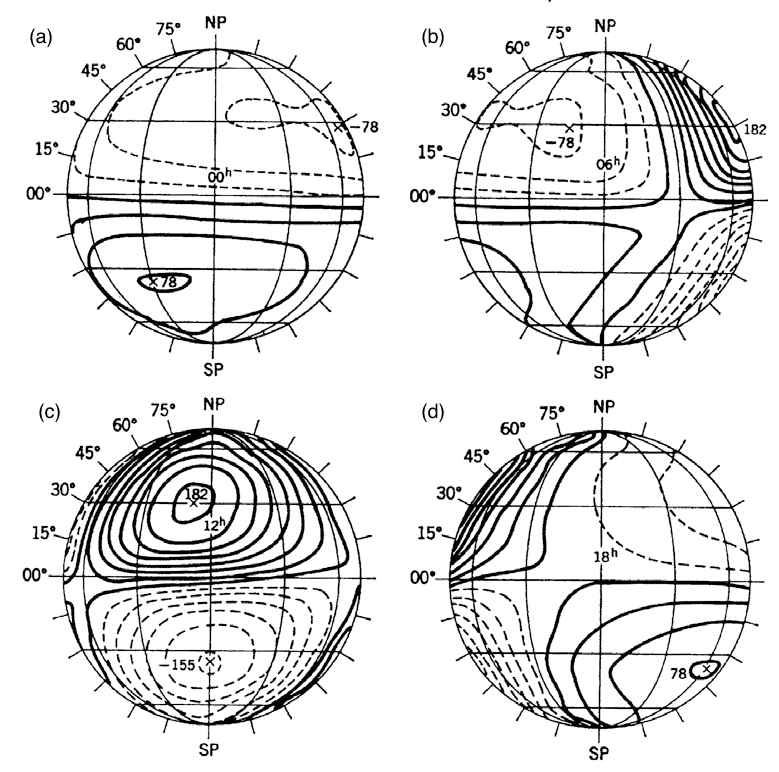
\includegraphics[width=.65\linewidth]{bilder/L3_solar_quiet.png}
    \caption{\(S_q\) current systems.}\label{fig:solar_quiet}
\end{figure}
We get geomagnetic pulsations when MHD waves enter the magnetic field. They make the field lines resonate since the field lines are fixed in the conducting ionosphere. Each field line has a natural resonating frequency which depends on field line length and plasma density profile along the field line.

\section{Magnetic \(L\)-value}
\begin{definition}[Magnetic \(L\)-value]\label{def:mag_L_value}
    The magnetic \(L\)-value describes the distance at which a particular magnetic field line crosses the equatorial plane.
\end{definition}
\noindent The magnetic \(L\)-value (sometimes called ``\(L\)-shell'') can be a convenient way to describe locations in geospace. It is derived from considering an observation point \(P\) on the Earth. We can trace a magnetic field line out to the equatorial plane. From \cref{fig:magnetic_L_value} we have that \(\gf{B}\) is always parallel to field line and the equation
\begin{equation*}
    \tan\alpha=B_\lambda/B_r=-\cos\lambda_m/2\sin\lambda_m=r\tn{d}\lambda_m/\tn{d}r
\end{equation*}
From this we get
\begin{equation*}
    \Rightarrow \frac{\tn{d}r}{r}=-2\frac{\sin\lambda_m}{\cos\lambda_m}\tn{d}\lambda_m
\end{equation*}
A solution to this equation is
\begin{equation*}
    \ln r=2\ln(\cos\lambda_m)+C
\end{equation*}
where \(C\) is an arbitrary constant of integration. When \(\lambda_m=0\) (equatorial plane) we have \(r=r_0\).
\begin{align*}
    \therefore C&=\ln r_0\\
    \therefore r&=r_0\cos^2\lambda_m
\end{align*}
For a plane on Earth’s surface (\(r=R_E\)) the field line through this point reaches the equatorial plane at distance
\begin{equation*}
    r_0=\frac{R_E}{\cos^2\lambda_m}
\end{equation*}
We define the ratio \(r_0/R_E=L\), i.e.\
\begin{equation*}
    L=\cos^{-2}\lambda_m\quad\Rightarrow\quad\lambda_m=\arccos\left(\sqrt{\frac{1}{L}}\right)
\end{equation*}
At Tromsø, \(\lambda_m=67\degree\Rightarrow \boxed{L=6.55}\) (\(r_0\approx 41730\si{\kilo\metre}\)).

\begin{figure}[t]
    \centering
    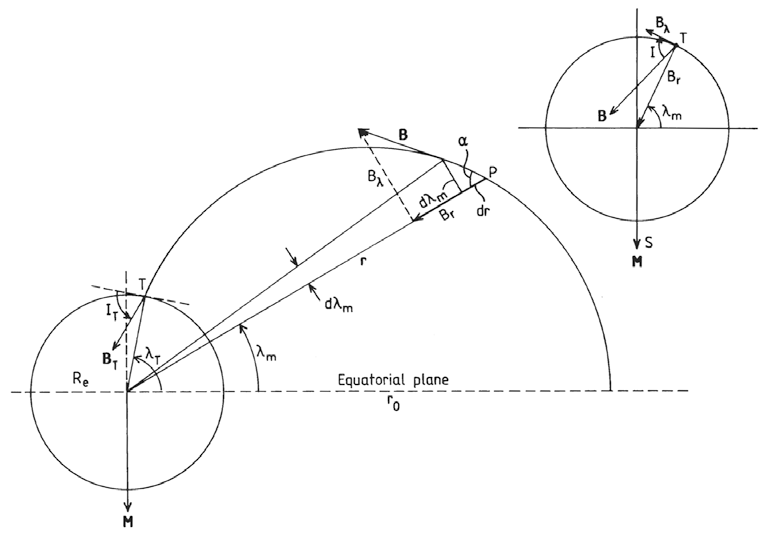
\includegraphics[width=.6\linewidth]{bilder/L3_magnetic_L_value.png}
    \caption{Magnetic \(L\)-value.}\label{fig:magnetic_L_value}
\end{figure}

\section{\(E\)-field mapping along conducting field lines}
We now look at how we can map the \(E\)-field, and our main assumption is that we have conducting field lines. We consider an electric field created in the ionosphere (\cref{fig:E_field_mapping}). We map this electric field into the equatorial plane. We will map the azimuthal and meridional components separately. We first consider two magnetic field lines separated in azimuth (\cref{fig:E_field_mapping1})
\begin{align*}
    \ell_{i\phi}&=\tn{ separation in ionosphere}\\
    L_{m\phi}&=\tn{ separation in equatorial plane}
\end{align*}
The separation is constant along geomagnetic latitudes.
\begin{equation*}
    \ell_{i\varphi}=R_E\cos\lambda_m\tn{d}\phi
\end{equation*}
\begin{equation*}
    L_{m\phi}=r_0\tn{d}\phi=\frac{R_E}{\cos^2\lambda_m}\tn{d}\phi
\end{equation*}
We assume that the line connecting the ionosphere to the equatorial plane is an equipotential
\begin{equation*}
    \Phi_\phi=E_{i\phi}\ell_{i\phi}=E_{m\phi}L_{m\phi}
\end{equation*}
where \(E_{i\phi}\) is the azimuthal component of \(\gf{E}\) in the ionosphere (equivalent for \(E_{m\phi}\)).
\begin{equation*}
    \frac{E_{i\phi}}{E_{m\phi}}=\frac{L_{m\phi}}{\ell_{i\phi}}=\frac{1}{\cos^3\lambda_m}=L^{3/2}
\end{equation*}
\textbf{E.g.}\ Tromsø: \(L\sim 6.5\Rightarrow \) enhancement of \(16.6\). Equatorial field of \(\SI{1}{\milli\volt\metre^{-1}}\) is enhanced to \(\SI{16.6}{\milli\volt\metre^{-1}}\) in the ionosphere.

We then look at two field lines separated in the meridian (\cref{fig:E_field_mapping2}). Consider two field lines separated by an angle \(\lambda_m\) in the meridional plane
\begin{align*}
    \ell_{i\lambda}&=\tn{ separation in ionosphere}\\
    L_{m\lambda}&=\tn{ separation in equatorial plane}
\end{align*}
From earlier, we have \(r_0=R_E/\cos^2\lambda_m\)
\begin{equation*}
    \ell_{i\varphi}=R_E\tn{d}\lambda_m\sin I
\end{equation*}
\begin{equation*}
    L_{m\phi}=\tn{d}r_0=2R_E\frac{\sin\lambda_m}{\cos^3\lambda_m}\tn{d}\lambda_m
\end{equation*}
The mapping ratio then become
\begin{align*}
    \frac{E_{i\lambda}}{E_{m\lambda}}&=\frac{L_{m\lambda}}{\ell_{i\lambda}}=\frac{2\sin\lambda_m}{\cos^3\lambda_m\sin I}\\
    &=\frac{2\sin\lambda_m}{\cos^3\lambda_m}\frac{1}{2\tan\lambda_m\cos I}\\
    &=\frac{1}{\cos^2\lambda_m}\frac{1}{\cos I}=\frac{1}{\cos^2\lambda_m}\sqrt{4\tan^2\lambda_m+1}\\
    &=L\sqrt{4\tan^2\lambda_m+1}=2L\sqrt{L-\frac{3}{4}}
\end{align*}
\textbf{E.g.}\ Tromsø: \(L=6.5\Rightarrow \) mapping ratio \(=31.2\). Equatorial field of \(\SI{1}{\milli\volt\metre^{-1}}\) is enhanced to \(\SI{31.2}{\milli\volt\metre^{-1}}\) in the ionosphere.

\begin{figure}[t]
    \centering

    \begin{subfigure}[t]{.49\linewidth}
        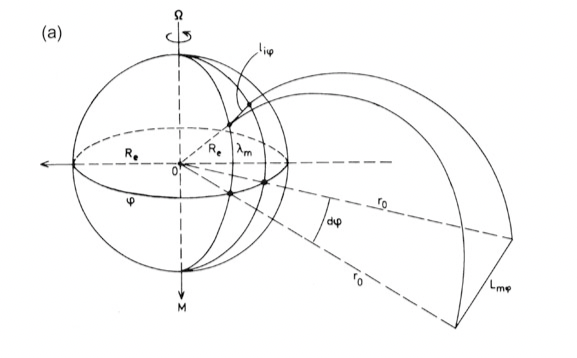
\includegraphics[width=.95\linewidth]{bilder/L3_E_field_mapping.png}
        \caption{}\label{fig:E_field_mapping1}
    \end{subfigure}
    \begin{subfigure}[t]{.49\linewidth}
        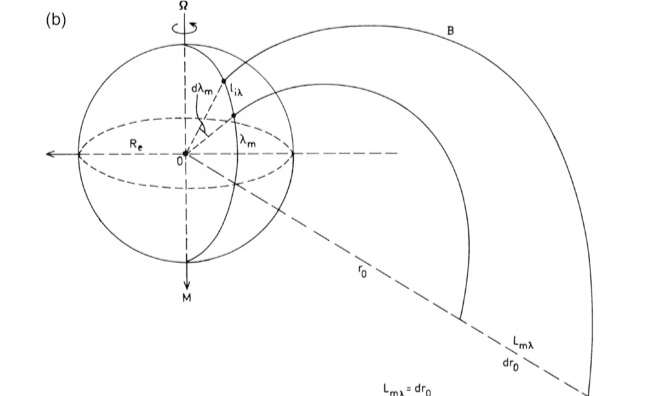
\includegraphics[width=.95\linewidth]{bilder/L3_E_field_mapping2.png}
        \caption{}\label{fig:E_field_mapping2}
    \end{subfigure}

    \caption{\(E\)-field mapping along conducting field lines.}\label{fig:E_field_mapping}
\end{figure}